\documentclass[9pt,a5paper]{extarticle}
\usepackage[margin=1cm]{geometry}
\usepackage[utf8]{inputenc}
\usepackage[IL2]{fontenc}
\usepackage[czech]{babel}
\usepackage{microtype}
\usepackage{amssymb}
\usepackage{amsthm}
\usepackage{amsmath}
\usepackage{xcolor}
\usepackage{graphicx}
\usepackage{wasysym}
\usepackage{multicol}

\usepackage[inline]{enumitem}

\newcommand{\R}{\mathbb{R}}

\newcommand{\hint}[1]{{\color{gray}\footnotesize\noindent(Nápověda: #1)}}

\DeclareMathOperator{\tg}{tg}
\DeclareMathOperator{\cotg}{cotg}

\setlist[enumerate]{label={(\alph*)},topsep=\smallskipamount,itemsep=\smallskipamount,parsep=0pt,itemjoin=\quad}
\setlist[itemize]{topsep=\smallskipamount,noitemsep}

\def\tisk{%
\newbox\shipouthackbox
\pdfpagewidth=2\pdfpagewidth
\let\oldshipout=\shipout
\def\shipout{\afterassignment\zdvojtmp \setbox\shipouthackbox=}%
\def\zdvojtmp{\aftergroup\zdvoj}%
\def\zdvoj{%
    \oldshipout\vbox{\hbox{%
        \copy\shipouthackbox
        \hskip\dimexpr .5\pdfpagewidth-\wd\shipouthackbox\relax
        \box\shipouthackbox
    }}%
}}%



\newtheorem*{poz}{Pozorování}

\theoremstyle{definition}
\newtheorem{uloha}{\atr Úloha}
\newtheorem{suloha}[uloha]{\llap{$\star$ }Úloha}
\newtheorem*{bonus}{Bonus}
\newtheorem*{defn}{Definice}

\pagestyle{empty}

\DeclareMathOperator{\arctg}{arctg}

\let\ee\expandafter

\def\vysld{}
\let\printvysl\relax

\makeatletter
\long\def\vyslplain#1{\ee\ee\ee\gdef\ee\ee\ee\vysld\ee\ee\ee{\ee\vysld\ee\printvysl\ee{\the\c@uloha}{#1}}}
\let\vysl\vyslplain

\def\locvysl#1{\ee\gdef\ee\locvysld\ee{\locvysld\item #1}}
\let\lv\locvysl

\newenvironment{ulohav}[1][]{\begin{uloha}[#1]\gdef\locvysld{\begin{enumerate*}}}{\ee\vyslplain\ee{\locvysld\end{enumerate*}}\end{uloha}}
\def\stitem{\@noitemargtrue\@item[$\star$ \@itemlabel]}

\makeatother

\def\atr{}
\def\basic{\def\atr{\llap{\mdseries$\sun$ }\gdef\atr{}}}
\def\interest{\def\atr{\llap{$\star$ }\gdef\atr{}}}

\begin{document}

%\tisk

\section*{13. Determinanty všeho druhu}


\begin{ulohav}\label{nuda}
Spočtete následující velmi zajímavé determinanty:
\begin{flushleft}
\begin{enumerate*}[itemjoin=\qquad]
    \item $\begin{vmatrix}3 & 4 \\ 2 & -5\end{vmatrix}$\lv{$-23$}
    \item $\begin{vmatrix}2 &3 & 1 \\ -1 & 2 & 3 \\ 3 & 2 & -1\end{vmatrix}$\lv{$0$}
    \item $\begin{vmatrix}1 &1 & 2 \\ 2 & 3 & 1 \\ 3 & 4 & -5\end{vmatrix}$\lv{$-8$}
    \item $\begin{vmatrix}\sqrt2&\sqrt3&\sqrt6 \\ \sqrt6&\sqrt2&\sqrt3 \\ \sqrt3&\sqrt6&\sqrt3\end{vmatrix}$\lv{$5 \sqrt{3}+3 \sqrt{6}-12$}
\end{enumerate*}
\end{flushleft}
\end{ulohav}


\begin{uloha}
Spočtěte obsah trojúhelníka $ABC$, který má vrcholy v bodech o souřadnicích $A[1; 2]$, $B[2; 5]$ a $C[5; 6]$. \hint{Trojúhelník je \uv{polovina} rovnoběžníka.}\vyslplain{4}
\end{uloha}


\begin{ulohav}
Rovnoběžnostěn $ABCDEFGH$ má vrcholy v bodech o souřadnicích $A[0;0;0]$, $B[1;1;2]$, $D[2;3;1]$, $E[3;4;-5]$.
\begin{enumerate}
    \item Určete souřadnice zbývajících čtyř vrcholů.\lv{$C[3;4;3]$, $F[4;5;-3]$, $G[6;8;-2]$, $H[5;7;-4]$}
    \item Určete objem onoho rovnoběžnostěnu.\lv{$8$}
    \item Určete objem (nepravidelného) čtyřstěnu $ABDE$.\lv{$\frac16 \cdot 8 = \frac43$} \hint{Jakou část rovnoběžnostěnu tvoří čtyřstěn? Jak by to bylo pro kvádr?}
\end{enumerate}
\end{ulohav}


\begin{ulohav}
Nalezněte všechna reálná $x$, aby platilo
\begin{flushleft}
\begin{enumerate*}[itemjoin=\qquad]
    \item $\begin{vmatrix}6 & 2 \\ 3 & x\end{vmatrix} = 0$\lv{$x=1$}
    \item $\begin{vmatrix}8 & 6 & 4 \\ x & 5 & 5 \\ 7 & x & x-2\end{vmatrix} = 0$\lv{$x_1 = 1$, $x_2 = 5$}
\end{enumerate*}
\end{flushleft}
\end{ulohav}


\begin{uloha}
Určete všechna reálná čísla $x$ tak, aby trojúhelník s vrcholy o souřadnicích $A[1; 2]$, $B[2; 5]$ a $C[x; x+1]$ měl obsah 4.\vysl{$x_1 = -3$, $x_2 = 5$}
\end{uloha}


\interest
\begin{uloha}
Určete objem naprosto nepravidelného mnohostěnu $ABCDE$, jehož vrcholy mají souřadnice $A[1; 2; 3]$, $B[4; 5; 6]$, $C[-1; 4; 3]$, $D[5; 2; 1]$, $E[-3; 7; -3]$.
\hint{Podívejte se na obrázek a rozdělte mnohostěn na dva vhodné čtyřstěny.}
\[ 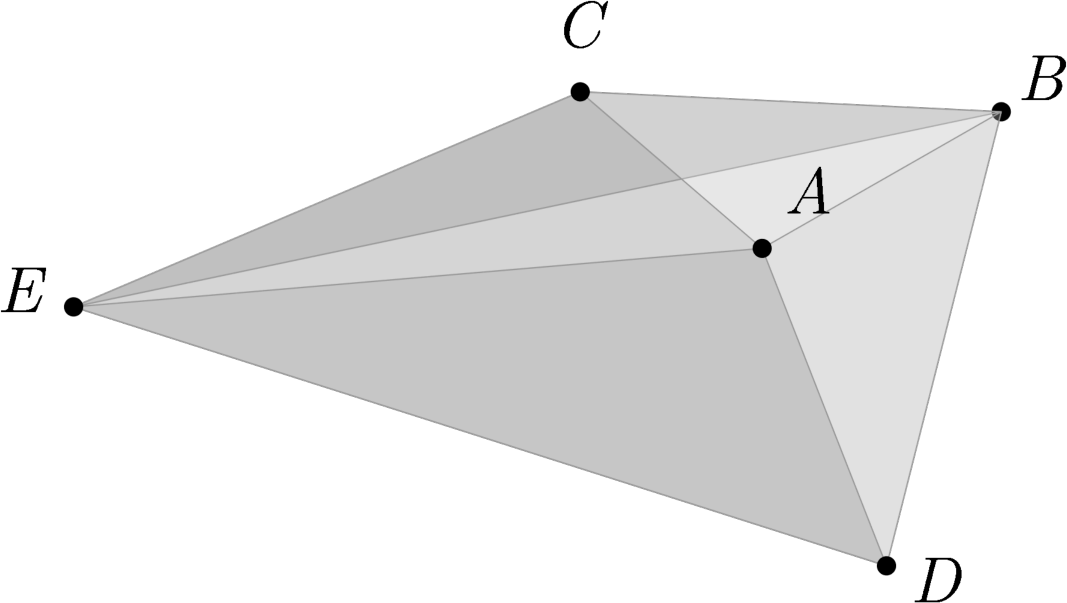
\includegraphics[width=5.4cm]{mnohosten.png} \]\vyslplain{44 ($ABEC$ má objem 13 a $ABED$ 31)}
\end{uloha}


\interest
\begin{uloha}
Rozmyslete si následující:
\begin{enumerate}
    \item \emph{Transpozice}, tj. následující operace \uv{záměny řádků a sloupců}
    \[ \begin{vmatrix}a&b\\c&d\end{vmatrix}\mapsto\begin{vmatrix}a&c\\b&d\end{vmatrix},\qquad \begin{vmatrix}a&b&c\\d&e&f\\g&h&i\end{vmatrix} \mapsto \begin{vmatrix}a&d&g\\b&e&h\\c&f&i\end{vmatrix} \]
    nezmění hodnotu determinantu.
    \item Prohození dvou řádků (sloupců) v determinantu změní jeho znaménko.
    \item Když celý jeden řádek (sloupec) vynásobíme nějakým číslem, výsledný determinant se taky tímto číslem vynásobí.
    \stitem Když k jednomu řádku (sloupci) přičteme libovolný násobek jiného řádku (sloupce), hodnota determinantu se nezmění.
\end{enumerate}
\end{uloha}


\newpage
\parindent=0pt
\parskip=\smallskipamount
\def\printvysl#1#2{\textbf{#1.} #2\par}
\vysld


\end{document}